% *********************************************************************
% © 2021–2026 Jeremy Sylvestre
%
% Permission is granted to copy, distribute and/or modify this document
% under the terms of the GNU Free Documentation License, Version 1.3 or
% any later version published by the Free Software Foundation; with no
% Invariant Sections, no Front-Cover Texts, and no Back-Cover Texts. A
% copy of the license is included in the appendix entitled “GNU Free
% Documentation License” that appears in the output document of this
% PreTeXt source code. All trademarks™ are the registered® marks of
% their respective owners.
%
% *********************************************************************

\newcommand*{\xmin}{0.5}
\newcommand*{\xmax}{6}
\newcommand*{\ymin}{-5}
\newcommand*{\ymax}{5}
\newcommand*{\func}{\x * \x * \x - 9 * \x * \x + 23 * \x - 14}

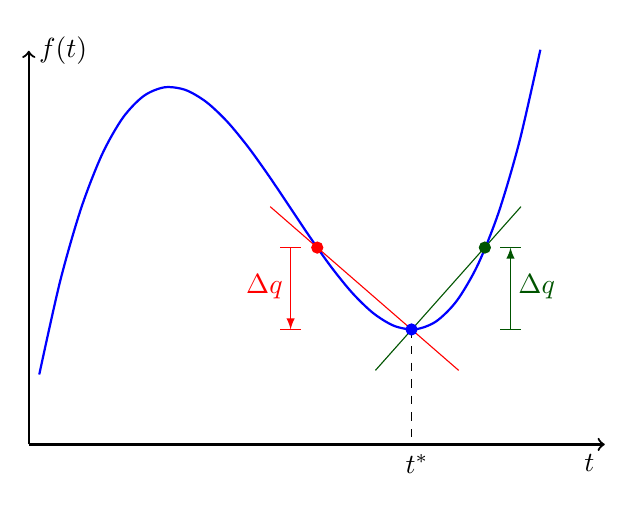
\begin{tikzpicture}
[
	closedpt/.style={circle,draw,fill,inner sep=0pt,minimum size=4pt},
	openpt/.style={circle,draw,inner sep=0pt,minimum size=4pt},
	xscale=1.33,
	yscale=0.5
]

	% axes
	\draw[->,thick] (\xmin,\ymin) -- (\xmax,\ymin) node[below left] {$t$};
	\draw[->,thick] (0.5,\ymin) -- (0.5,\ymax) node[right] {$f(t)$};

	\draw[red] (2.805,1.04) -- (4.605,-3.119);
	\draw[red]
	  (2.9,0) -- (3.1,0)
	  (2.9,-2.079) -- (3.1,-2.079)
	;
	\draw[red,-latex] (3,0) -- (3,-2.079);
	\node[red] at (2.75,-1) {$\Delta q$};

	\draw[green!33!black] (5.2,1.04) -- (3.81,-3.119);
	\draw[green!33!black]
	  (5,0) -- (5.2,0)
	  (5,-2.079) -- (5.2,-2.079)
	;
	\draw[green!33!black,-latex] (5.1,-2.079) -- (5.1,0);
	\node[green!33!black] at (5.35,-1) {$\Delta q$};

	% example graph
	\draw[blue, thick, domain=0.6:5.385, smooth] plot (\x,{\func});

	\draw[dashed] (4.1547,-2.079) -- (4.1547,\ymin) node[below,xshift=0.07cm] {$t^\ast$};

	\node[blue,closedpt] at (4.1547, -2.079) {};
	\node[red,closedpt] at (3.2547, 0) {};
	\node[green!33!black,closedpt] at (4.855, 0) {};

\end{tikzpicture}
